\documentclass[aspectratio=169]{beamer} %format: 16:9


\usepackage[american]{babel}

\usetheme{ITD1}
\withoutframelogo

\usepackage{csquotes}
\usepackage{derivative}
\usepackage[
  backend=biber,
  doi=true,
  eprint=false,
  date=iso,
  seconds=true,
  style=alphabetic-verb,
  locallabelwidth=true,
  maxnames = 99,
  %citestyle=alphabetic-verb
  ]{biblatex}
\renewcommand*{\bibfont}{\footnotesize}

\addbibresource{literature.bib}




\title{An Experimental Analysis of the Influence of the Precision of Parameters in an Artificial Neural Network}

% CHANGE IDX HERE
\subtitle{Natural Computation PS Presentation 01}

\author[D. K., E. R., S. A. S., L. S.]{Denise Katritschenko, Elias Reich, Sayed Abozar Sadat, Lukas Schwaiger}
\institute[\plusshort]{\pluslong\\ Department of Artificial Intelligence and Human Interfaces (AIHI)}
\date[\today]{\today}


\AtBeginSection[]{\fullframe{\insertsectionhead}}



\begin{document}


\frame{\titlepage}


\section{Introduction}


% each frame is a 'slide'
\begin{frame}{Primer on Neural Networks}
  \begin{figure}
    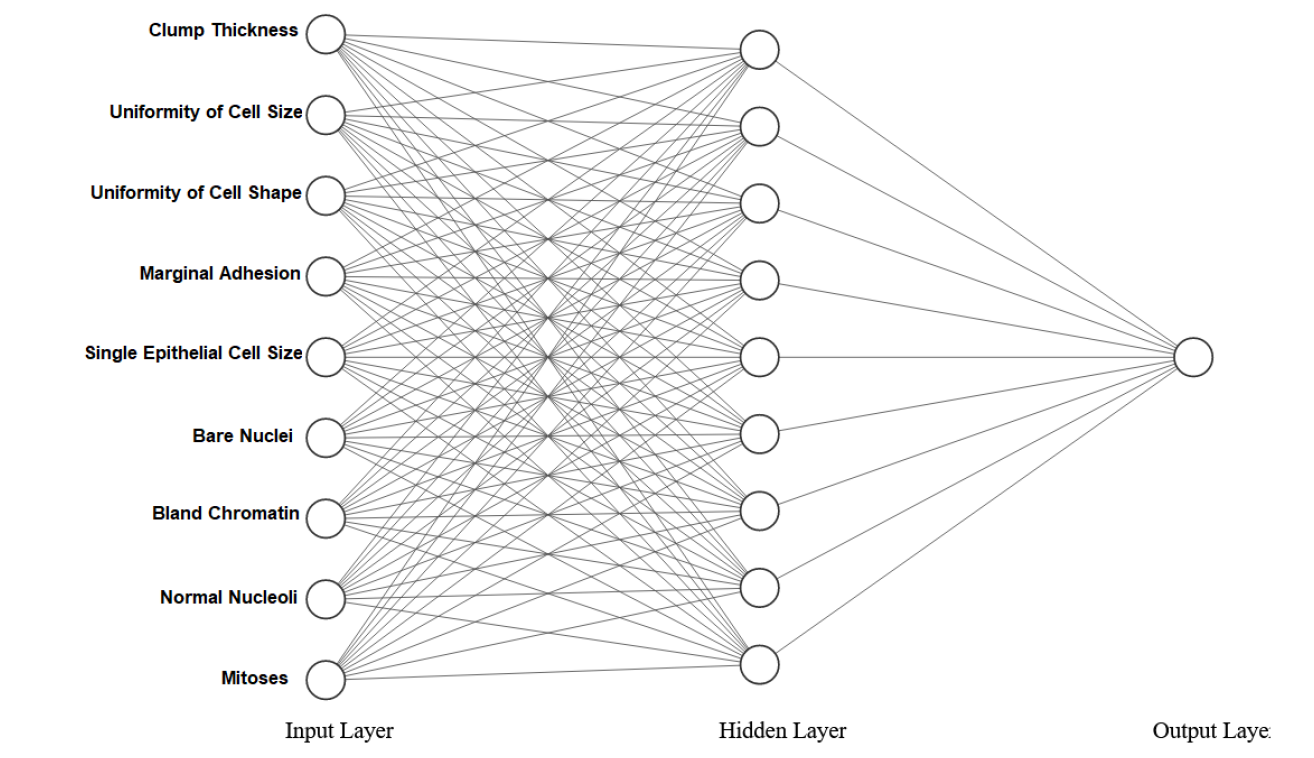
\includegraphics[width=0.7\textwidth]{figures/mlp.png}
    \caption{Example png.}
  \end{figure}
\end{frame}


\begin{frame}{Single neuron view}
  \begin{figure}
    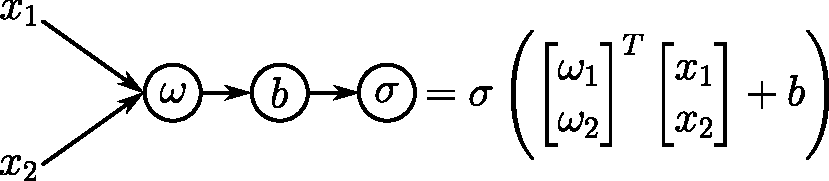
\includegraphics[width=0.96\textwidth]{figures/single-neuron.pdf}
    \caption{Example pdf.}
  \end{figure}

  You can still add more here.
\end{frame}


\begin{frame}{Gradients}
  \begin{itemize}
    \item Want to optimize the parameters $\omega$ and $b$.
    \item Need a target $y$ and error metric (loss $L$) to judge the networks predictions $\hat y$.
    \item Convex optimization is used to adjust the parameters.
    \item Many intermediate results need to be stored for efficient gradient computation.
  \end{itemize}

  \begin{align*}
    L(f(x_1, x_2)) &= (\sigma(\omega^T x + b) - y) ^2\\
                   &= (\sigma(a) - y) ^ 2\\
                   &= (\hat y - y) ^ 2
  \end{align*}
  \begin{alignat*}{3}
    \pdv{L}{\omega_1} &= \pdv{L}{\sigma} &&\pdv{\sigma}{a}      &&\pdv{a}{\omega_1}\\
                      &= 2(\hat y - y)~~ &&\odv{}{a}\sigma(a)~~ &&x_1
  \end{alignat*}
  
\end{frame}


\begin{frame}
  Frame without title.\\

  Example citation~\cite{Russel2020}.
\end{frame}


\begin{skipframecount}

\begin{frame}[allowframebreaks]{References}
  \printbibliography[heading=none]
\end{frame}

\appendix

\end{skipframecount}


\end{document}
